%% LaTeX Beamer presentation template (requires beamer package)
%% see http://bitbucket.org/rivanvx/beamer/wiki/Home
%% idea contributed by H. Turgut Uyar
%% template based on a template by Till Tantau
%% this template is still evolving - it might differ in future releases!

\documentclass{beamer}

\mode<presentation>
{
\usetheme{Warsaw}

\setbeamercovered{transparent}
}

\usepackage[english]{babel}
\usepackage[latin1]{inputenc}

% font definitions, try \usepackage{ae} instead of the following
% three lines if you don't like this look
\usepackage{mathptmx}
\usepackage[scaled=.90]{helvet}
\usepackage{courier}

\usepackage[T1]{fontenc}

% User packages
\usepackage[absolute,overlay]{textpos}
\usepackage{tikz}
\usepackage{listings}

\title{Birdhouse - supporting Web Processing Services}

%\subtitle{}

% - Use the \inst{?} command only if the authors have different
%   affiliation.
\author{\vspace{2.3cm}\\
Carsten Ehbrecht\inst{1}
%\and J.~M.~de~Jesus\inst{2}
}
%\author{\inst{1}}

% - Use the \inst command only if there are several affiliations.
% - Keep it simple, no one is interested in your street address.
\institute[Universities of]
{
\inst{1}%
DKRZ - German Climate Compute Center
%\and
%\inst{2}%
%GeoCAT
}

\date{\footnotesize{$9^{th}$ of November / Python Frameworks Conference 2017}}


% This is only inserted into the PDF information catalog. Can be left
% out.
\subject{Talks}



% If you have a file called "university-logo-filename.xxx", where xxx
% is a graphic format that can be processed by latex or pdflatex,
% resp., then you can add a logo as follows:

% \pgfdeclareimage[height=0.5cm]{university-logo}{university-logo-filename}
% \logo{\pgfuseimage{university-logo}}



% Delete this, if you do not want the table of contents to pop up at
% the beginning of each subsection:
\AtBeginSubsection[]
{
\begin{frame}<beamer>
\frametitle{Outline}
\tableofcontents[currentsection,currentsubsection]
\end{frame}
}

% Section title slides
\AtBeginSection[]{
  \begin{frame}
  \vfill
  \centering
  \begin{beamercolorbox}[sep=8pt,center,shadow=true,rounded=true]{title}
    \usebeamerfont{title}\insertsectionhead\par%
  \end{beamercolorbox}
  \vfill
  \end{frame}
}


% If you wish to uncover everything in a step-wise fashion, uncomment
% the following command:

%\beamerdefaultoverlayspecification{<+->}

\begin{document}

\begin{frame}
   \tikz [remember picture,overlay]
    \node at
        ([yshift=4.8cm]current page.south)
        %or: (current page.center)
        {
\includegraphics[height=2.8cm]{figures/pywps}};
   \titlepage
\end{frame}

\begin{frame}
\frametitle{Outline}
\tableofcontents
% You might wish to add the option [pausesections]
\end{frame}

% %%%%%%%%%%%%%%%%%%%%%%%%%%%%%%%%%%%%%%%%%%%%%%%%%%%%%%%%%%%%%%%%%%%%%%%%%%%%%
\section{Introduction}

%\subsection[Short First Subsection Name]{First Subsection Name}

% -----------------------------------------------
\begin{frame}
\frametitle{PyWPS 4.0 is finally here}
%\framesubtitle{Subtitles are optional}

\begin{itemize}
  \item Over three years in development \pause
  \item Relevant contributions by over a dozen individuals \pause
  \item New licence: MIT \pause
  \item OSGeo accreditation around the corner \ldots
\end{itemize}
\end{frame}



% -----------------------------------------------
\begin{frame}
\frametitle{What is PyWPS?}

\begin{itemize}
  \item An implementation of the OGC Web Processing Service standard \pause
\item Coded on the Python language (researcher friendly)  \pause
\item Started in the Spring of 2006  \pause
\item Supports all available tools in Python for geo-spatial operations  \pause
\item http://pywps.org

\end{itemize}
\end{frame}


% -----------------------------------------------
\begin{frame}
\frametitle{What PyWPS is not}

\begin{itemize}
  \item Complicated  \pause
  \item A client  \pause
  \item A GUI or any other user interface  \pause
  \item a server with pre-installed processes
\end{itemize}

\end{frame}



% -----------------------------------------------
\begin{frame}
\frametitle{What is PyWPS good for?}

\begin{itemize}
  \item Make your models available to the world  \pause
  \item Enables remote processing of complex and/or lengthy models  \pause
  \item Guarantees model inputs fit basic requirements
        (e.g. type, number)  \pause
  \item Guarantees interoperability of model inputs and outputs
  \begin{itemize}
    \item using the OGC data standards
	\item formalizing input/output data types
  \end{itemize}
\end{itemize}
\end{frame}


% %%%%%%%%%%%%%%%%%%%%%%%%%%%%%%%%%%%%%%%%%%%%%%%%%%%%%%%%%%%%%%%%%%%%%%%%%%%%%
\section{OGC Web Processing Service}

% -----------------------------------------------
\begin{frame}
\frametitle<presentation>{The OGC Web Processing Service}

\begin{itemize}
\item OGC open web standard for remote geo-spatial processing.  \pause
\item Integrated with web data services: \textbf{WFS}, \textbf{WCS}.  \pause
\item Three basic requests:
\begin{itemize}
      \item  \textit{GetCapabilities}
      \item  \textit{DescribeProcess}
      \item  \textit{Execute}   \pause
\end{itemize}
\item Three basic input/output classes:
\begin{itemize}
      \item  \textit{Literal}
      \item  \textit{Complex} - for geo-spatial data and services
      \item  \textit{BoundingBox} - for geo-spatial data extent
\end{itemize}
\end{itemize}
\end{frame}



% -----------------------------------------------
\begin{frame}
\frametitle<presentation>{The OGC Web Processing Service}

  \begin{figure}[ht]
   \centering
   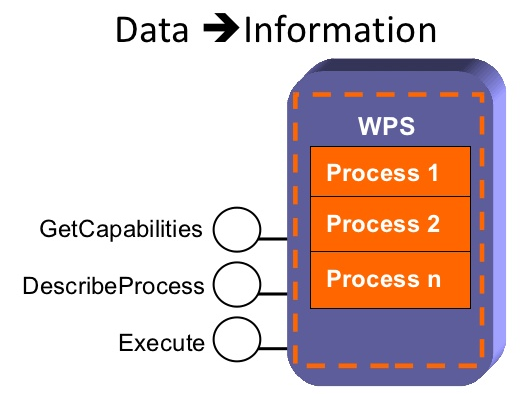
\includegraphics[height=5.85cm]{figures/WPS}
  \end{figure}

\centering
\footnotesize{http://www.slideshare.net/TheodorFoerster/restful-web-processing-service}

\end{frame}


% %%%%%%%%%%%%%%%%%%%%%%%%%%%%%%%%%%%%%%%%%%%%%%%%%%%%%%%%%%%%%%%%%%%%%%%%%%%%%
\section{Summary}

\begin{frame}
\frametitle<presentation>{Summary}

\begin{itemize}
  \pause
  \item SQLAlchemy
  \begin{itemize}
    \item Improved logging
    \item Powerful process management becomes possible
    \item Support to many different database systems
    \item \textit{Ad hoc} logging from user processes \ldots
  \end{itemize}
  \pause
  \item Deployment
  \begin{itemize}
    \item Nginx + Gunicorn provide the infrastructure for scalable services
    \item Scalability implies increased complexity
  \end{itemize}
  \pause
  \item{Docker containers}
  \begin{itemize}
    \item dockerfiles create pre-configured PyWPS images
    \item set up and deployment complexity already in place
  \end{itemize}
\end{itemize}

\end{frame}

% --------------------------------------------------------------
\begin{frame}
%\frametitle<presentation>{}

  \begin{figure}[ht]
   \centering
   
\includegraphics[height=3cm]{figures/pywps}
  \end{figure}

\centering
\Huge{Thank you!}

\vspace{0.4cm}
\normalsize{www.pywps.org}
\end{frame}

\end{document}
